%
% pie.tex
%
\renewcommand{\thisname}{Chart::Pie}
\section{\thisname}
\name{\thisname}
\file{Pie.pm}
\requires{Chart::Base, GD, Carp, FileHandle}
\begin{Description}
The class \thisclass creates a pie chart. The first added set must
contain the labels, the second set the values. \thisclass is a subclass
of \class{Chart::Base}.
\end{Description}

\example
\begin{figure}[ht]
  \begin{center}
    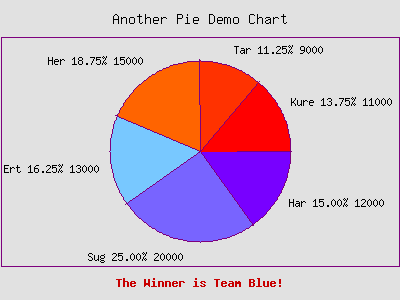
\includegraphics[scale = 0.6]{d_pie3.png}
  \end{center}
  \caption{Pie chart}
  \label{fig:pie}
\end{figure}
\begin{verbatim}
use Chart::Pie;

$g = Chart::Pie->new();

$g->add_dataset('Har', 'Sug', 'Ert', 'Her', 'Tar', 'Kure');
$g->add_dataset(12000, 20000 , 13000, 15000, 9000, 11000  );

%opt = ('title'        => 'Another Pie Demo Chart',
        'label_values' => 'both',
        'legend'       => 'none',
        'text_space'   => 10,
        'png_border'   => 1,
        'graph_border' => 0,
        'colors' => { 'x_label'    => 'red',
                      'misc'       => 'plum',
                      'background' => 'grey',
                      'dataset0'   => [120, 0, 255],
                      'dataset1'   => [120, 100, 255],
                      'dataset2'   => [120, 200, 255],
                      'dataset3'   => [255, 100, 0],
                      'dataset4'   => [255, 50, 0],
                      'dataset5'   => [255, 0, 0],
                    },
        'x_label'      => 'The Winner is Team Blue!',
       );

$g->set(%opt);

$g->png("pie.png");
\end{verbatim}

\constructorblurb{\thisname}

\begin{AttrDecl}{label\_values}
Tells \thisclass what kind of value labels to show alongside the pie.
Valid values are \literal{percent}, \literal{value}, \literal{both} and
\literal{none}. Defaults to \literal{percent}.
\end{AttrDecl}

\begin{AttrDecl}{legend\_label\_values}
Tells \thisclass what kind of labels to show in the legend. Valid values
are \literal{percent}, \literal{value}, \literal{both} and
\literal{none}. Defaults to \literal{value}.
\end{AttrDecl}

\begin{AttrDecl}{legend\_lines}
The labels drawn alongside the pie are connected with a line to the
segment if this option is set to \literal{true}.
\end{AttrDecl}

\begin{AttrDecl}{ring}
The pie can have a ring shape instead of the usual disc shape. This
option determines the thickness of the ring as a fraction of the radius.
Default is 1, \ie, a full pie.
\end{AttrDecl}
